\section{Introduction}
\begin{frame}
\frametitle{Introduction}
\end{frame}

% **************************************************
% HIGH-PERFORMANCE COMPUTING
% **************************************************
\subsection*{High-performance computing}
\begin{frame}
\frametitle{High-performance computing}

\begin{itemize}
\pause
\item Increasing need for computational power
\pause
\item Grids and cloud computing
\pause
\item Many-core systems
\end{itemize}
\vspace{10pt}

\pause
Many computaions running on high-performing systems do not make use of
the performance available.
\vspace{10pt}

\pause
We need software that achieves \emph{strong scaling}.

\end{frame}


% **************************************************
% COPERNICUS
% **************************************************
\subsection*{Copernicus}
\begin{frame}
\frametitle{Copernicus}
\framesubtitle{What is Copernicus?}

Copernicus is a software system that was originally made to distribute
and parallelize large molecular simulations.
\vspace{10pt}

\pause
It shares attributes with cloud computing.
\end{frame}


\begin{frame}
\frametitle{Copernicus}
\framesubtitle{Architecture}

\begin{columns}
  \column{0.5\textwidth} An example Copernicus architecture with two
  project servers and four network servers.
  \vspace{10pt}

  \pause Clusters 0 and 1 may be located in A with a common gateway
  server, while cluster 2 is located at B.

  \column{0.5\textwidth}
  \begin{figure}
    \centering
    \includegraphics[width=\textwidth]{gfx/arch.pdf}
  \end{figure}
\end{columns}

\end{frame}


\begin{frame}
\frametitle{Copernicus}
\framesubtitle{Network model}

\begin{columns}
  \column{0.5\textwidth} The nonbonded kernels use SIMD assembly and
  each Copernicus task is a massively parallel message-passing
  simulation.
  \vspace{10pt}

  \pause Beyond the point of efficiently scaling individual
  simulations, hundreds of workers are employed on a typical cluster
  or supercomputer, and these communicate with other resources through
  additional servers.
  \vspace{10pt}

  \pause Top-level servers interact with controllers, or project
  servers, to determine what tasks to execute.

  \column{0.5\textwidth}
  \begin{figure}
    \centering
    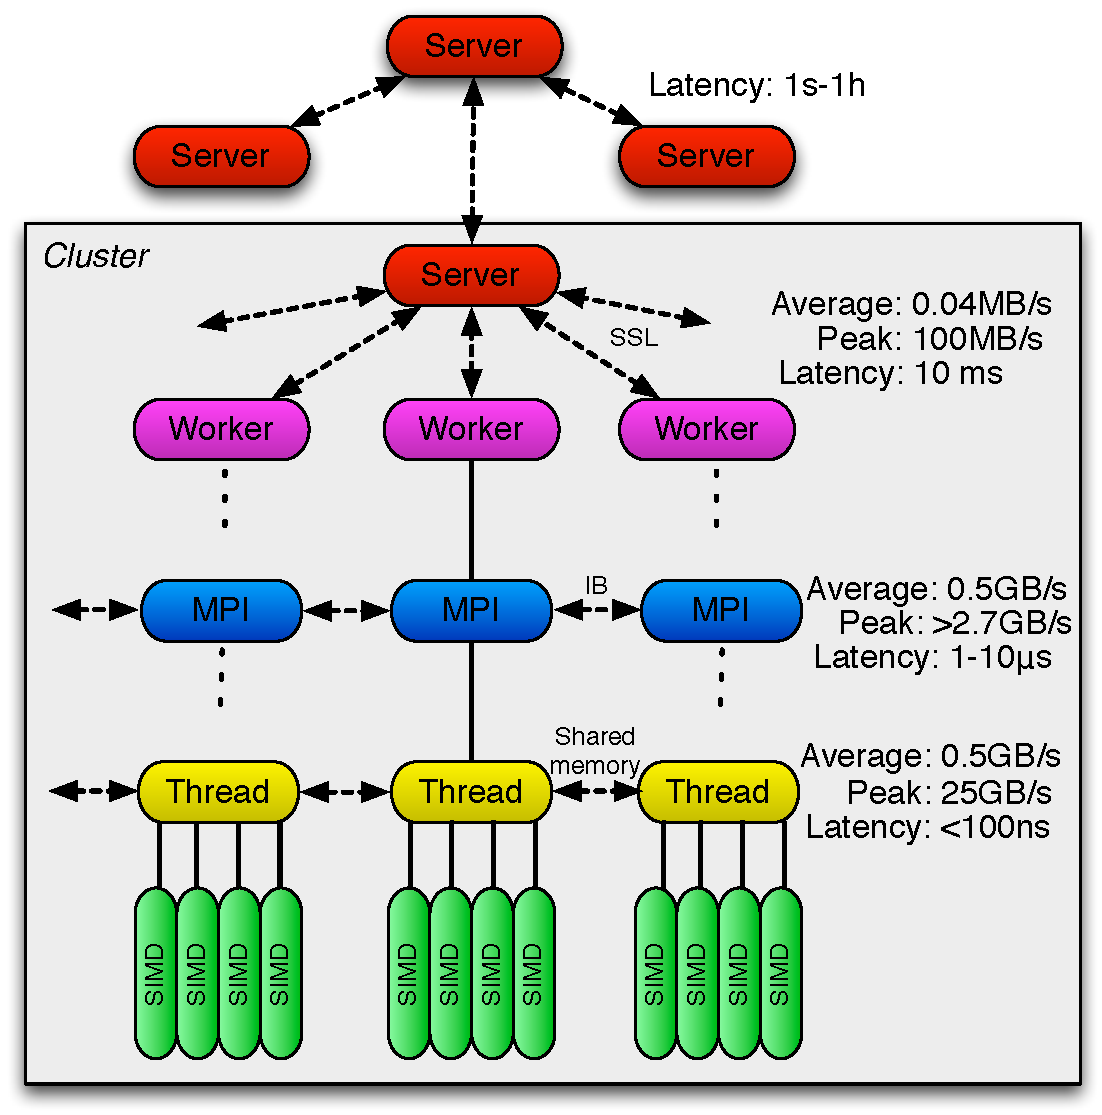
\includegraphics[width=\textwidth]{gfx/parallelization.pdf}
  \end{figure}
\end{columns}

\end{frame}


% **************************************************
% PROBLEM STATEMENT
% **************************************************
\subsection*{Problem statement}
\begin{frame}
\frametitle{Problem statement}

The aim of our project was to design a suitable input
description-language for Copernicus.

\end{frame}
